% Native PGFPlots; reproduced by examples/generate_foundation_figures.py.
% Constructed observations / analytical teaching example, not empirical data.
\begingroup
\definecolor{blueplot}{HTML}{4E79A7}
\definecolor{redplot}{HTML}{D95F59}
\definecolor{inkplot}{HTML}{111111}
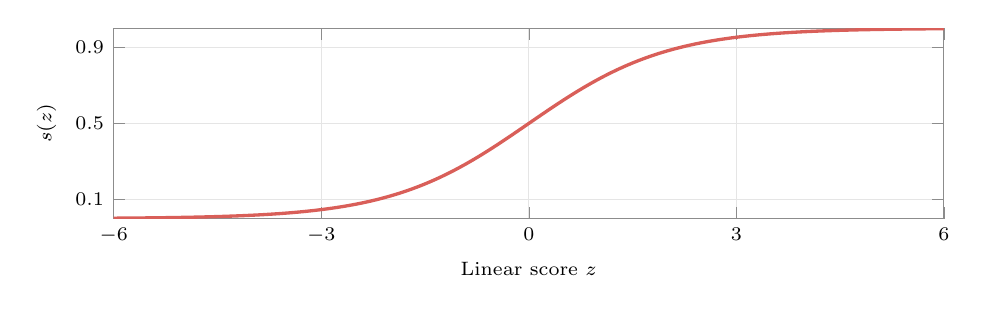
\begin{tikzpicture}
\begin{axis}[
width=\linewidth,height=4.0cm,font=\scriptsize,
tick label style={font=\scriptsize},label style={font=\scriptsize},
axis line style={black!45},tick style={black!45},
grid=major,grid style={black!10},scaled ticks=false,
clip=true,unbounded coords=jump,
legend style={font=\tiny,draw=none,fill=white,fill opacity=.94,text opacity=1,
  legend cell align=left,inner sep=2pt,row sep=1pt},
xmin=-6,xmax=6,ymin=0,ymax=1,
xlabel={Linear score $z$},ylabel={$\operatorname{s}(z)$},
xtick={-6,-3,0,3,6},ytick={.1,.5,.9}
]
\addplot[redplot,very thick,no marks] coordinates {(-6,0.002472623157) (-5.9,0.002731960763) (-5.8,0.003018416325) (-5.7,0.003334807307) (-5.6,0.003684239899) (-5.5,0.004070137716) (-5.4,0.004496273161) (-5.3,0.00496680165) (-5.2,0.005486298899) (-5.1,0.006059801492) (-5,0.006692850924) (-4.9,0.007391541344) (-4.8,0.008162571153) (-4.7,0.009013298653) (-4.6,0.009951801867) (-4.5,0.01098694263) (-4.4,0.01212843498) (-4.3,0.01338691783) (-4.2,0.01477403169) (-4.1,0.01630249937) (-4,0.01798620996) (-3.9,0.01984030573) (-3.8,0.02188127094) (-3.7,0.02412702142) (-3.6,0.02659699358) (-3.5,0.02931223075) (-3.4,0.0322954647) (-3.3,0.03557118927) (-3.2,0.0391657228) (-3.1,0.04310725494) (-3,0.04742587318) (-2.9,0.05215356308) (-2.8,0.0573241759) (-2.7,0.06297335606) (-2.6,0.06913842034) (-2.5,0.07585818002) (-2.4,0.08317269649) (-2.3,0.09112296101) (-2.2,0.09975048912) (-2.1,0.1090968212) (-2,0.119202922) (-1.9,0.1301084744) (-1.8,0.1418510649) (-1.7,0.1544652651) (-1.6,0.1679816149) (-1.5,0.1824255238) (-1.4,0.1978161114) (-1.3,0.214165017) (-1.2,0.2314752165) (-1.1,0.2497398944) (-1,0.2689414214) (-0.9,0.2890504974) (-0.8,0.3100255189) (-0.7,0.3318122278) (-0.6,0.3543436938) (-0.5,0.3775406688) (-0.4,0.4013123399) (-0.3,0.4255574832) (-0.2,0.4501660027) (-0.1,0.4750208125) (0,0.5) (0.1,0.5249791875) (0.2,0.5498339973) (0.3,0.5744425168) (0.4,0.5986876601) (0.5,0.6224593312) (0.6,0.6456563062) (0.7,0.6681877722) (0.8,0.6899744811) (0.9,0.7109495026) (1,0.7310585786) (1.1,0.7502601056) (1.2,0.7685247835) (1.3,0.785834983) (1.4,0.8021838886) (1.5,0.8175744762) (1.6,0.8320183851) (1.7,0.8455347349) (1.8,0.8581489351) (1.9,0.8698915256) (2,0.880797078) (2.1,0.8909031788) (2.2,0.9002495109) (2.3,0.908877039) (2.4,0.9168273035) (2.5,0.92414182) (2.6,0.9308615797) (2.7,0.9370266439) (2.8,0.9426758241) (2.9,0.9478464369) (3,0.9525741268) (3.1,0.9568927451) (3.2,0.9608342772) (3.3,0.9644288107) (3.4,0.9677045353) (3.5,0.9706877692) (3.6,0.9734030064) (3.7,0.9758729786) (3.8,0.9781187291) (3.9,0.9801596943) (4,0.98201379) (4.1,0.9836975006) (4.2,0.9852259683) (4.3,0.9866130822) (4.4,0.987871565) (4.5,0.9890130574) (4.6,0.9900481981) (4.7,0.9909867013) (4.8,0.9918374288) (4.9,0.9926084587) (5,0.9933071491) (5.1,0.9939401985) (5.2,0.9945137011) (5.3,0.9950331983) (5.4,0.9955037268) (5.5,0.9959298623) (5.6,0.9963157601) (5.7,0.9966651927) (5.8,0.9969815837) (5.9,0.9972680392) (6,0.9975273768)};

\end{axis}
\end{tikzpicture}
\endgroup
